\documentclass[a4paper]{article}

\usepackage{color}
\usepackage{url}
\usepackage[T2A]{fontenc} % enable Cyrillic fonts
\usepackage[utf8]{inputenc} % make weird characters work
\usepackage{graphicx}


\usepackage[unicode]{hyperref}
\hypersetup{colorlinks,citecolor=green,filecolor=green,linkcolor=blue,urlcolor=blue}

%\newtheorem{primer}{Пример}[section] %ćirilični primer
\newtheorem{primer}{Primer}[section]

\title{Reklame na društvenim mrežama\\ \small{Seminarski rad u okviru kursa\\Tehničko i naučno pisanje\\ Matematički fakultet}}

\author{Natalija Pavlićević (pavlicevicnatalija@gmail.com)\\ Teodora Maksimović (teamax18@gmail.com)\\ Branka Marković (bakymarkovic@gmail.com)\\ Mihailo Damnjanović (mihailo.damnjanović@gmail.com)}
\date{15.~novembar 2022.}
\maketitle
\begin{document}
	
	\abstract{Ovo je apstrakt za ovaj seminarski rad.
	}
	
	\tableofcontents
	
	\newpage
	
	\section{Reklamiranje na društvenim mrežama}
	\label{sec:uvod}
	Reklamiranje na društvenim mrežama je vrsta digitalnog marketinga koja koristi društvene mreže za isporuku plaćenih oglasa ciljnoj grupi ljudi. Oglasi na društvenim mrežama su efektivan način povezivanja sa potrošačima. Koristeći različite izvore podataka oglašivači su u mogućnosti da isporuče personalizovani sadržaj. Kada se publika upozna sa određenim brendom na društvenim mrežama oglašivači mogu da vrše interakcije sa potrošačima. Oglasi na društvenim mrežama su takođe uglavnom isplativi I imaju potencijal za visoke stope povraćaja. Reklame na društvenim mrežama su neophodne za kompanije ako žele da dođu do novih ciljanih tržišta. 
	
	\section{Prikupljanje podataka korisnika u cilju personalizovanog oglašavanja}
	\label{sec:podaci}
	Ciljano reklamiranje je sve veća oblast interesovanja za i poslovne i istraživačke zajednice. Reklame u mobilnim uslugama i oglasi u aplikaciji predstavljaju oblast rasta u nastajanju, u kojoj ciljano reklamiranje postaje sve važniji izvor prihoda i za oglašivače i za reklamne kompanije. Oglašivači sve više koriste personalizovano reklamiranje koje je prilagođeno potrošačima na osnovu podataka koji se tiču njihovih preferencija i ponašanja, a koje dobijaju prikupljanjem njihovih ličnih podataka koji se obrađuju za svrhe profilisanja i ciljanja. Podaci koje pružaju korisnici omogućavaju onlajn provajderima društvenih medija da personalizuju svoj sadržaj. Personalizacijom oni ciljaju na relevantniji oglasni sadržaj s jedne strane i ostvaruju veći profit za oglašivače s druge strane, čineći oglase efikasnijim i ciljanijim.
	Društvene mreže su mesto u kom danas ljudi slobodno izražavaju emocije. One prikupljaju podatke u strukturisanim i nestrukturisanim, formalnim i neformalnim podacima. Okupljeni podaci sadrže osećanja i mišljenja korisnika koji će biti obrađeni tehnikama rudarenja podataka i analizirani za postizanje smislenih informacija iz njega. Koristeći podatke društvenih medija možemo klasifikovati tip korisnika analizom njihovih objavljenih podataka na društvenim veb stranicama. Svi ovi podaci sadrže ključne reči koje igraju glavnu ulogu kad se radi o oglašavanju ciljanoj grupi ljudi.
	
	\subsection{Kolačići}
	\label{subsec:kolacici}
	Kolačići (formalnije HTTP kolačići) su male količine podataka sa nekog veb sajta koje se skladište na računaru korisnika dok on pretražuje taj veb sajt. Kolačići imaju mnoge funkcije kao što su praćenje aktivnosti korisnika kako bi mu se prikazale ciljane informacije kao što su oglasi za robu ili usluge. Na primer ako pretražujemo maskice za telefon na Amazonu, kasnije tog dana možemo videti oglase za maskice na Fejsbuku. Kolačići takođe mogu imati I druge uloge kao što je pamćenje podataka za prijavu za određenu veb stranicu tako da možete da je zatvorite a zatim da je ponovo otvorite bez potrebe za ponovnim prijavljivanjem. Kolačići takođe pružaju vlasnicima sajta informacije o tome koliko različitih korisnika je posetilo njihov sajt u određenom periodu. To je moguće jer svaki kolačić ima sopstveni ID, pa ako jedan korisnik poseti sajt više puta, kolačić nam omogućava da ga vidimo kao jednog jedinstvenog korisnika. Na taj način vlasnici veb stranica dobijaju preciznije informacije o saobraćaju na njima.
	
	\subsection{Vrste kolačića}
	\label{subsec:vrstekolacica}
	\textbf{Sesijski kolačići.} Sesijski kolačići pomažu veb stranici da prati sesiju korisnika. Sesijski kolačići se brišu kada korisnik napusti veb sajt ili se odjavi sa svog naloga. Sesijski kolačići nemaju rok trajanja, pa se brišu kad se sesija završi. 
	
	\textbf{Trajni kolačići.} Trajni kolačići uvek sadrže rok trajanja I za razliku od sesijskih kolačića ostaju u pregledaču unapred određeno vreme. 
	
	\textbf{Kolačići za autentifikaciju.} Kolačići za autentifikaciju pomažu u upravljanju korisničkim sesijama. Služe za to da se osetljive informacije prenesu do pravih korisničkih sesija povezivanjem informacija o korisničkom nalogu sa nizom identifikatora kolačića. 
	
	\textbf{Kolačići za praćenje.} Kolačići za praćenje generišu se preko usluga za praćenje. Oni pamte aktivnosti korisnika, a pregledači šalju te informacije usluzi za praćenje sledeći put kada se učita veb sajt koji koristi tu uslugu praćenja. 
	
	\textbf{Zombi kolačići.} Zombi kolačići se regenerišu nakon brisanja. Oni kreiraju svoje rezervne verzije izvan svog uobičajenog mesta za čuvanje. Nakon toga rezervne kopije se koriste kako bi se ponovo pojavile u pregledaču nakon brisanja. Zombi kolačiće obično koriste nesavesni oglasni servisi kao I sajber napadači 
	
	\textbf{Kolačići treće strane.} Kolačići treće strane se obično koriste u cilju praćenja korisnika. Za razliku od kolačića prve strane oni pripadaju domenu koji nije prikazan u pretraživaču. Na primer ako vršimo kupovinu na jednom sajtu, izvorni server tog sajta koristi sesijski kolačić kako bi zapamtio prijavljivanje korisnika na svoj nalog. To je primer kolačića prve strane. Međutim kolačić nekog drugog sajta može biti uskladišten u pretraživaču I pratiti aktivnost na prvom sajtu iako trenutno drugi sajt nije otvoren. To je primer kolačića treće strane. 
	
	\section{Algoritmi u odabiru reklama}
	\label{sec:algoritmi}
	Zašto mi Gugl (eng.~{\em Google}) i Fejsbuk (eng.~{\em Facebook}) nekad predlažu baš ono o čemu razmišljam? Kako to oni mogu uopšte znati? Odgovor glasi: algoritmi. Svakodnevno, upotrebom društvenih mreža, susrećemo se sa reklamama u različitim oblicima. Međutim, 		kako funkcioniše algoritam koji personalizuje reklamni sadržaj za svakog korisnika zasebno?\\ \\
	Postoji nešto što se zove trag na internetu (eng. digital footprint) i baš kao što i sam naziv kaže ukazuje na činjenicu da se svaki naš korak na internetu posmatra, prati, meri, beleži i čuva. Kako je tehnologija napredovala, u stopu su je pratili i algoritmi koji ove podatke 		obrađuju pa tako oni danas obrađuju sve do najsitnijih detalja – od toga na šta smo kliknuli ali i šta smo ignorisali, koliko smo se sekundi, minuta ili sati zadržali na svakom sadržaju. Sve ovo čini konstantan priliv podataka u sistem koji je potpuno mašinski osamostaljen tj. ne 		zahteva nadzor čoveka, a u cilju personalizacije sadržaja. Neke društvene mreže pružaju opciju pregleda zašto nam se neki oglas prikazuje. Primer za to je na slici \ref{fig:zastoreklama} : 
	\begin{figure}[h!]
		\begin{center}
			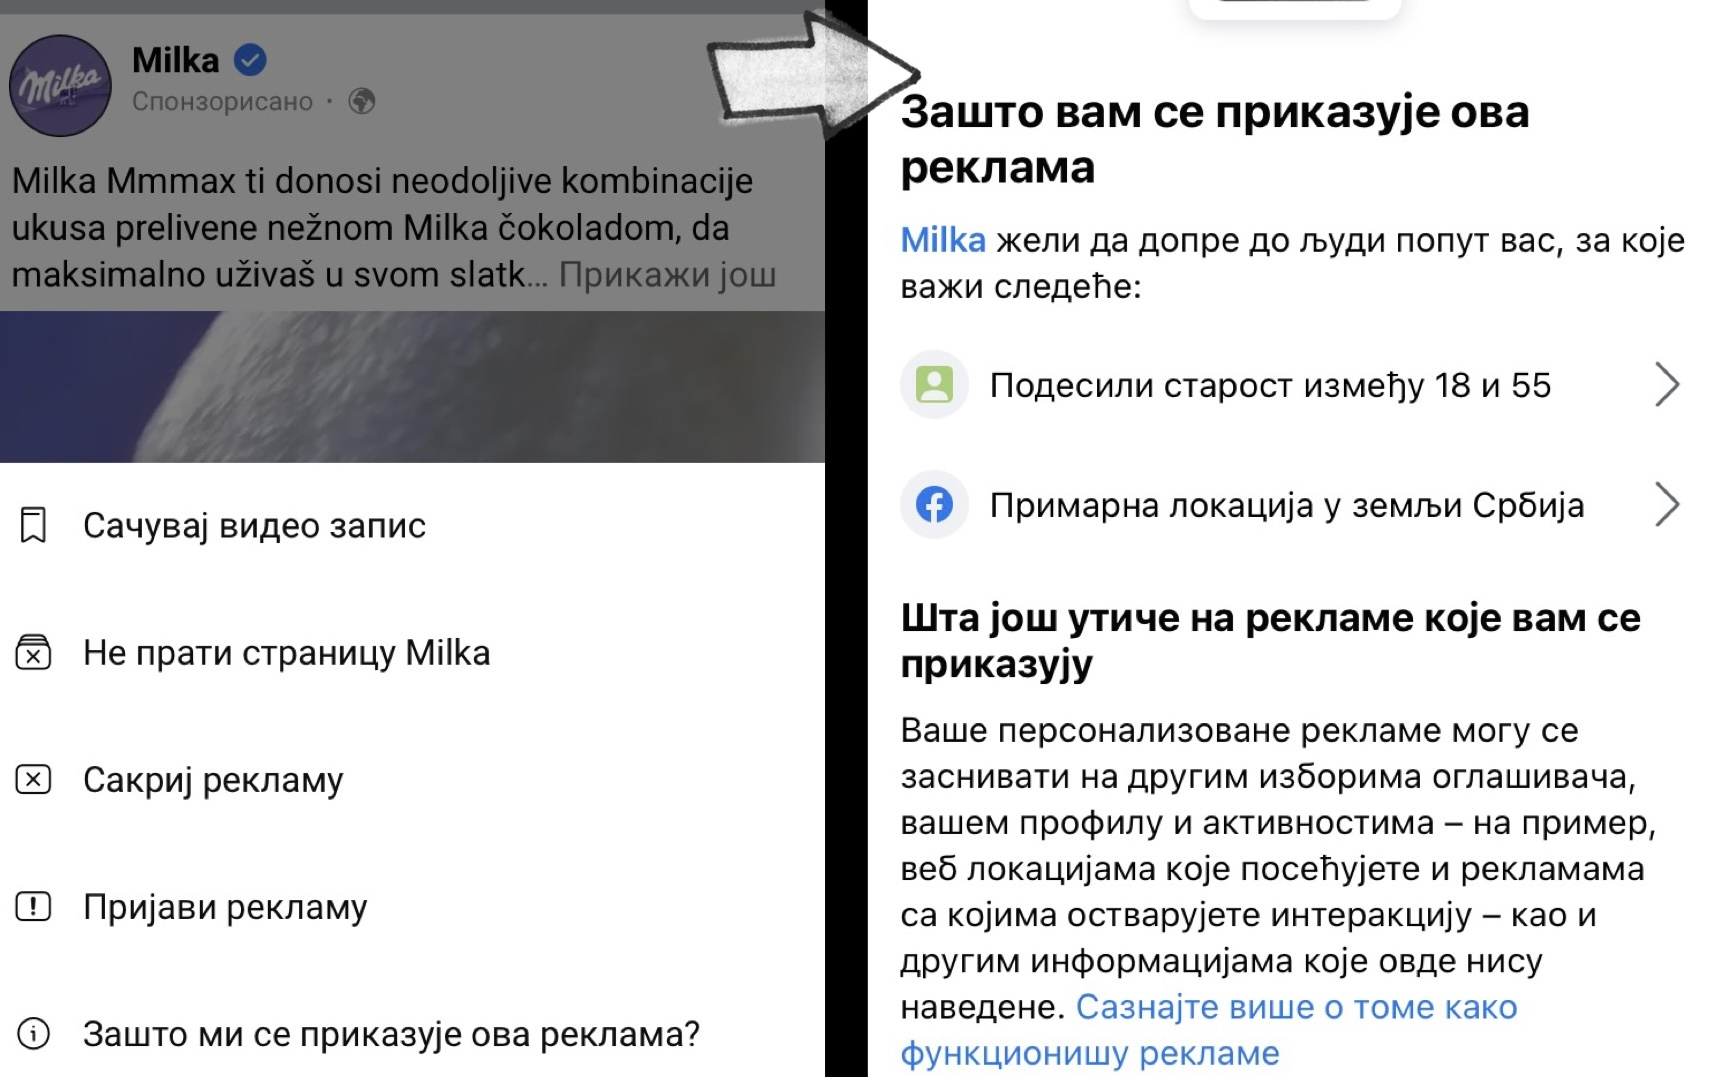
\includegraphics[scale=0.1]{zastoreklama.jpg}
		\end{center}
		\caption{Poruka Fejsbuka o prikazivanju reklame}
		\label{fig:zastoreklama}
	\end{figure}\\
	Imajući sve ove prikupljene podatke, svaka platforma nudi personalizovane reklame.  U oglašavanju, algoritam društvenih medija bira i bira oglase za koje misli da će korisnici biti zainteresovani da ih vide, na osnovu kvaliteta oglasa, načina na koji je oglas podesio njegov 		oglašivač (kao što je na koju demografsku kategoriju treba da cilja) i korisnikove prethodne interakcije sa sličnim tipom oglasa.  \cite{algoritmi}
	
	\subsection{Kako ovaj algoritam doprinosi uspešnosti reklama?}
	\label{subsec:uspesnostreklama}
	Ključna reč koju nam ovaj sistem obrade podataka pruža je personalizacija. Zašto? Pa, količina sadržaja objavljenog na društvenim mrežama svakog minuta je zapanjujuća. Da bi se izračunao najsmisleniji plaćeni sadržaj, algoritmi se koriste u pokušaju da kontrolišu bujicu 		informacija i prikazuju korisnicima samo sadržaj i oglase do kojih im je zaista stalo i na koje će eventualno potrošiti pare.
	\subsubsection{Koliki efekat zapravo može da postigne personalizovan marketing?}
	O tome govore sledeći podaci \cite{statistikai}:
	\begin{itemize}
		\item Personalizovana komunikacija sa kupcem koja je relevantna i korisna uvećava profit od 10 do 30\%;
		\item Personalizacija doprinosi impulsivnoj kupovini: 49\% ljudi kupilo je proizvod koji nije planiralo zahvaljujući personalizovanoj preporuci brenda sa kojim su sarađivali;
		\item Personalizacija dovodi do smanjenja vraćanja robe: samo 5\% kupaca je vratilo ono što je kupilo usled impulsivne kupovine, dok je čak 85\% bilo zadovoljno time što je kupilo;
		\item Personalizacija povećava lojalnost: 45\% kupaca kaže da bi verovatno ponovilo kupovinu kod brenda koji im je ponudio personalizovanu uslugu.
	\end{itemize} 
	
	
	\section{Mišljenje korisnika o reklamama na internetu}
	\label{sec:misljenje}
	Kroz istraživanje o mišljenju korisnika za reklame na internetu, došli smo do zaključka da se mišljenja razlikuju i da ima korisnika kojima smetaju reklame, a ima i onih koji vole da kliknu i vide šta im se ponudi u reklami.
	Same reklame korisnicima mogu da smetaju prilikom korišćenja nekih aplikacija ili gledanja filmova,kao i na youtube-u dok slušaju muziku jer reklame samo iskaču.To korisnicima kvari događaj i oni samo preskaču te reklame.
	Međutim, naravno da ima korisnika i koji vole kad im iskoči neka reklama, naročito ako oni u tom trenutku tragaju za tim proizvodima koji se reklamiraju, oni klikću na reklame.
	\subsection{Da li korisnici veruju reklamama na internetu?}
	\label{subsec:veovanje_reklamama}
	Dosta korisnika veruje reklamama na internetu ali samo onim koji su provereni ili se pronalaze u njima.Naravno ima određeni broj korisnika koji ne veruje reklamama i oni misle da su te reklame samo prevare koje privlače korisnike da kupe proizvode koji nisu tako dobri kao na reklama.U nastavku možete videti tabelu \ref{tab:verovanje_reklamama} koliko procenata veruje,a koliko ne.
	
	\begin{table}[h!]
		\begin{center}
			\caption{Verovanje reklamama}
			\begin{tabular}{|c|c|} \hline
				Da, verujem&9\%\\ \hline
				Da, ali samo reklamama brendova koje poznajem&29\%\\ \hline
				Da, ali samo ako su mi relevantna i pronalazim se u njima&37\%\\ \hline
				Ne verujem reklamama na internetu&25\%\\ \hline
			\end{tabular}
			\label{tab:tabela1}
		\end{center}
	\end{table}
	
	
	Ovo istraživanje izvršeno je od strane Social Serbia 2020.
	\subsection{Koliko cesto korisnici klikcu na reklame?}
	\label{subsec:klik_na_reklamu}
	Zanimljiva činjenica kod ovoga jeste to da je veći procenat muškaraca koji često klikcu na reklame nego žena. U nastavku možete videti sliku \ref{fig:klik_na_reklamu} koliko često korisnici klikću na reklame.
	
	
	\begin{figure}[h!]
		\begin{center}
			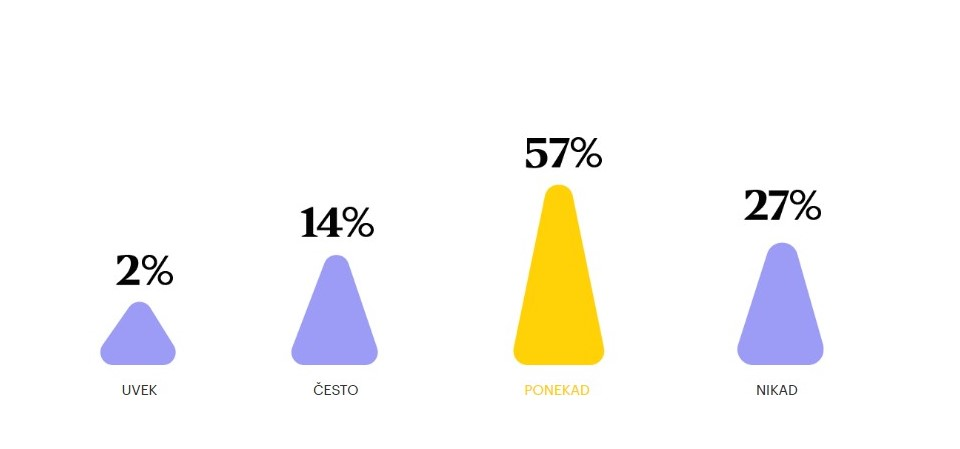
\includegraphics[scale=0.55]{klik_na_reklamu.jpg}
		\end{center}
		\caption{Klik na reklamu}
		\label{fig:klik_na_reklamu}
	\end{figure}
	Takođe i ovo istraživanje izvršeno je od strane Social Serbia 2022.
	\section{Doprinos od reklama}
	\label{sec:doprinos}
	Mnogi proizvođači se pitaju da li reklame doprinose prodaji ili ne.Doprinos je uglavnom veliki ukoliko se reklamirate na pravi način.Reklame na internetu u današnje vreme privuku najviše kupaca.
	\subsection{Da li se treba reklamirati?}
	\label{subsec:potrebna_reklama}
	Šta više uopšte se ne treba postavljati ovo pitanje.Prema istaraživanjima veliki procenat ljudi reklamira proizvode preko interneta, zato što su ljudi postali lenji i sve rade preko interneta.U nastavku možete videti listu o procentima doprinosa reklamiranja na internetu:
	1.84\% marketing stručnjaka se reklamira na nekoj društvenoj mreži
	2.83\% njih insistira da su društvene mreže bitne za njihov biznis
	3.Broj preduzetnika koji tvrde da je Facebook neophodan za njihov biznis je skocio na 75\%
	4.Društvene mreže su dovele do značajnog porasta stopi koverzije u poređenju sa tradicionalnim marketingom 
	Ovo istraživanje izvršeno je od stane hubspot marketing statistics.
	
	\newpage
	\addcontentsline{toc}{section}{Literatura}
	\appendix
	
	\iffalse
	\bibliography{seminarski} 
	\bibliographystyle{plain}
	\fi
	
	\begin{thebibliography}{9}
		
		\bibitem{marketingstatistics} Marketing statistics online at:https://www.hubspot.com/marketing-statistics
		
		\bibitem{socialserbia} Social Serbia 2020 online at:https://pioniri.com/sr/socialserbia2020/
		
		\bibitem{algoritmi}	Guide to social media ad algorithms online at https://digivizer.com/blog/your-guide-to-social-media-ad-algorithms/ 
		
		\bibitem{statistikai} Kako da ponudite kupcima personalizovano iskustvo kakvo žele online at https://www.biznis-akademija.com/blog/kako-da-ponudite-kupcima-personalizovano-iskustvo-kakvo-zele
		
		\bibitem{podaci} The Influence of Consumer–Brand Relationship on the Personalized Advertising Privacy Calculus in Social Media online at: https://www.sciencedirect.com/science/article/abs/pii/S1094996821000104        
		
		\bibitem{personalizacija} Investigating users’ experience on social media ads: perceptions of young users online at: https://www.sciencedirect.com/science/article/pii/S2405844020312226
		
		\bibitem{kolacici} What are cookies? | Cookies definition https://www.cloudflare.com/learning/privacy/what-are-cookies/
		
		
	\end{thebibliography}
	
	
	\appendix
\end{document}